\section{Test Examples}
\label{sec:test}

In order to better understand the results obtained in this section, it is worth to illustrate 
a link between classical PRA and RISMC approach.
Let's consider a system that is composed by two components (i.e, A and B) in a series configuration where
each component has a failure probability (i.e., $p_A$ and $p_B$ respectively) as shown in Fig.~\ref{fig:ABsystem}.

In a classical PRA framework such system can be modeled using a FT method that is composed by two basic events:
A failed and B failed.
System failure would be represented by a single ``AND'' gate that combine the two basic events as shown in 
Fig.~\ref{fig:ABsystem}.

In a RISMC approach, such system would be modeled by using two stochastic parameters (i.e., $var_A$ and $var_B$)
with a Bernoulli distribution $\operatorname{Bern}(p)$ associated to each of them: 
$var_A \sim \operatorname{Bern}(p_A)$ and $var_B \sim \operatorname{Bern}(p_B)$. 
The model that emulates system response would simply implement the ``AND" logic of the $var_A$ and $var_B$. 
In order to determine system failure probability a numerical integration has to be performed in a 2-dimensional 
(a dimension for each stochastic parameter).

Two possible sampling strategies can be followed:
\begin{itemize}
  \item Monte-Carlo: generate $N$ samples and count the the number of samples that lead to system failure
  \item Grid: partition the 2-dimensional space into a Cartesian grid; generate a sample for each partition 
        and associate a probability weight $w$ to each sample. This weight can be determined by integrating the pdf
        $pdf(A,B) = \operatorname{Bern}(p_A) \operatorname{Bern}(p_B)$ in each partition. 
        In this specific case, since each stochastic parameter 
        has two possible outcomes (i.e. 0 and 1), the space has been partitioned into 4 regions as 
        shown in Fig.~\ref{fig:2Danalogy}. Each cell of Fig.~\ref{fig:2Danalogy} has indicated the system outcome:
        system failure (F) or system success (OK).
\end{itemize}

The Monte-Carlo approach would require a large number of samples in order to decrease the statistical error associated
to system failure probability.
On the other hand, a Grid sampler would determine the exact value of system failure probability with only 4 samples:
\begin{enumerate}
  \item sample 1: $A=0$ and $B=0$ (bottom left cell of Fig.~\ref{fig:2Danalogy}), $w_1 = (1-p_A) \cdot (1-p_B)$
  \item sample 2: $A=1$ and $B=0$ (top left cell of Fig.~\ref{fig:2Danalogy}), $w_2 = p_A (1-p_B)$
  \item sample 3: $A=0$ and $B=1$ (bottom right cell of Fig.~\ref{fig:2Danalogy}), $w_3 = (1-p_A) \cdot p_B$
  \item sample 4: $A=1$ and $B=1$ (top right cell of Fig.~\ref{fig:2Danalogy}), $w_4 = p_A \cdot p_B$
\end{enumerate}
Note that each sample/cell of Fig.~\ref{fig:2Danalogy} that leads to system failure corresponds to a specific cut-set
\begin{itemize}
  \item Cut-set 1 (CS1) corresponds to sample 2; $p_{CS1} = p_A$
  \item Cut-set 2 (CS2) corresponds to sample 3; $p_{CS2} = p_B$
  \item Cut-set 3 (CS3) corresponds to sample 4; $p_{CS3} = p_A \cdot p_B$
\end{itemize}
Hence, the two methods (classical and PRA) would provide identical results.

Observe now that the number of samples required for $M$ stochastic parameters (assuming they are all distributed with 
a Bernoulli distribution) would be equal to $2^M$. Thus this strategy can be employed for a small value of $M$.

\begin{figure}
  \centering
  \begin{subfigure}{.5\textwidth}
    \centering
    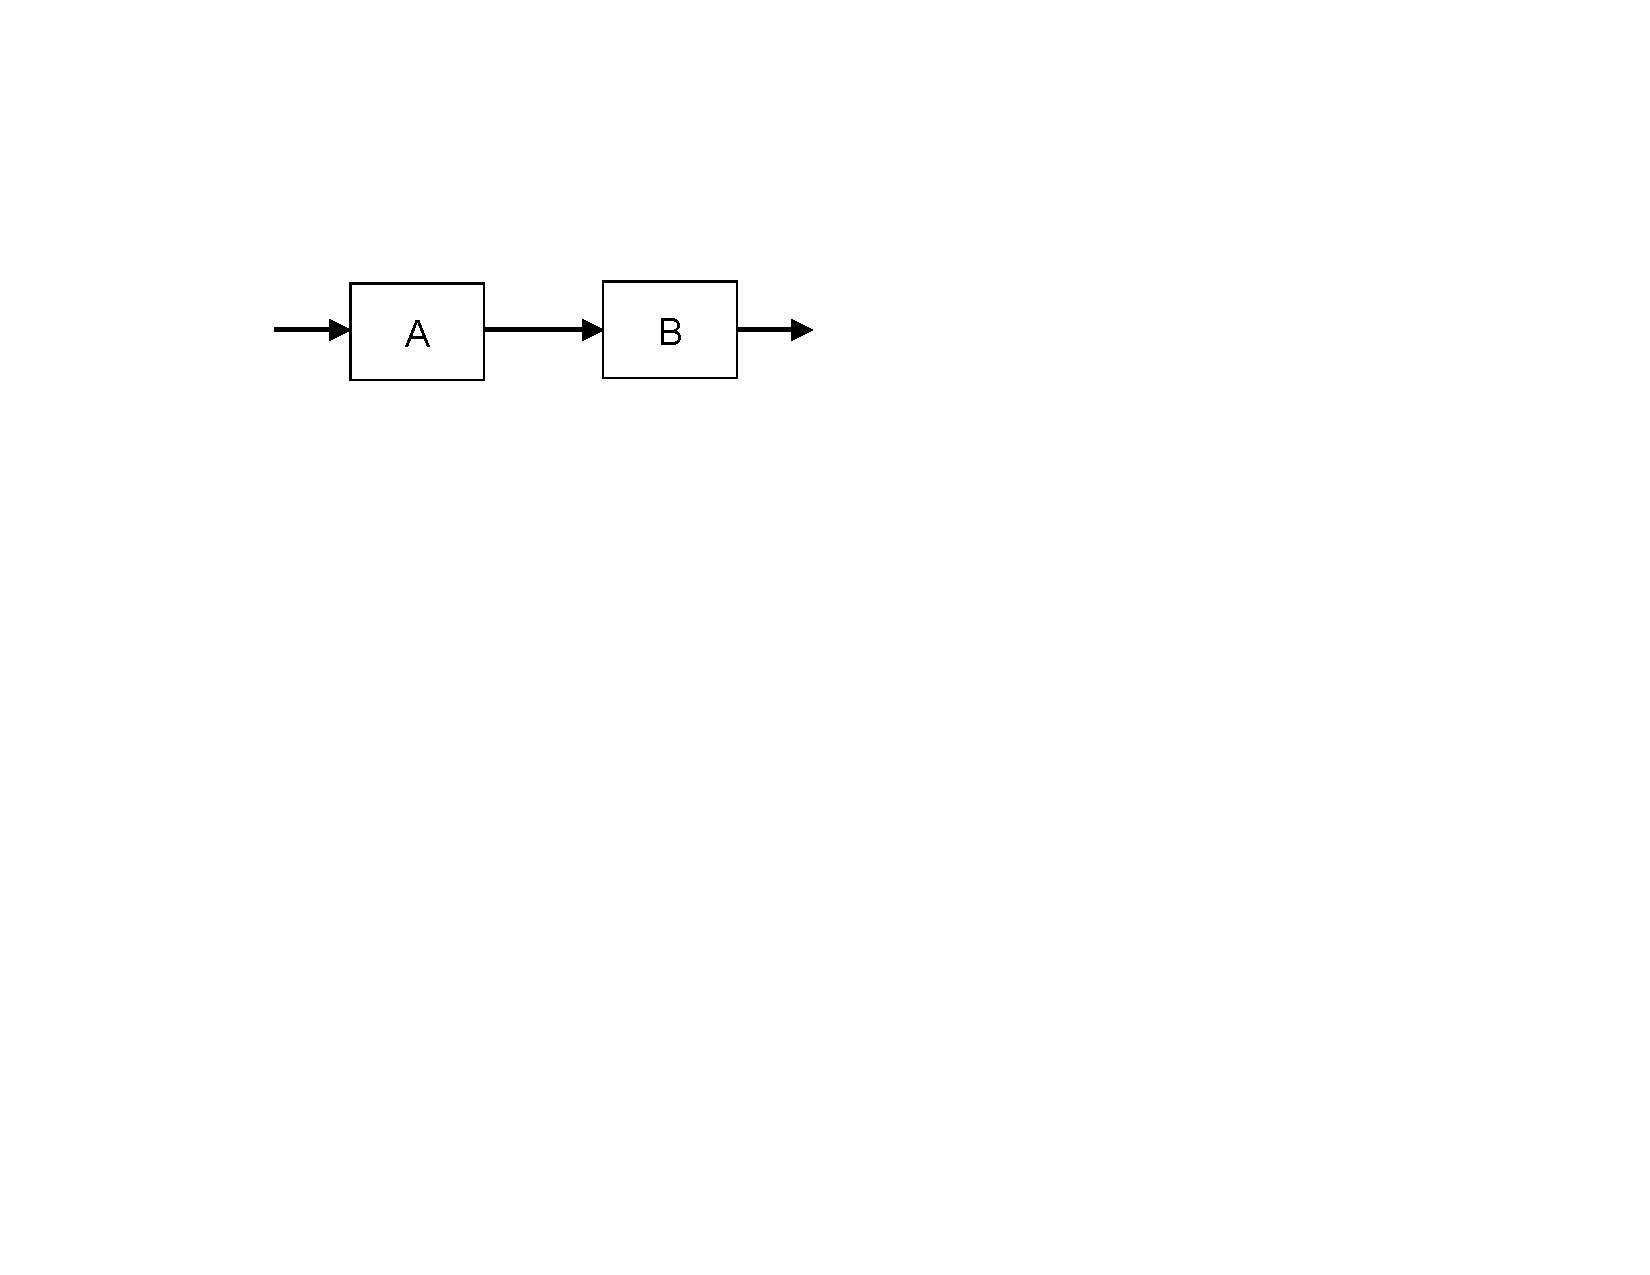
\includegraphics[scale=0.6]{ABsystem.pdf}
    \label{fig:sub1}
  \end{subfigure}%
  \begin{subfigure}{.5\textwidth}
    \centering
    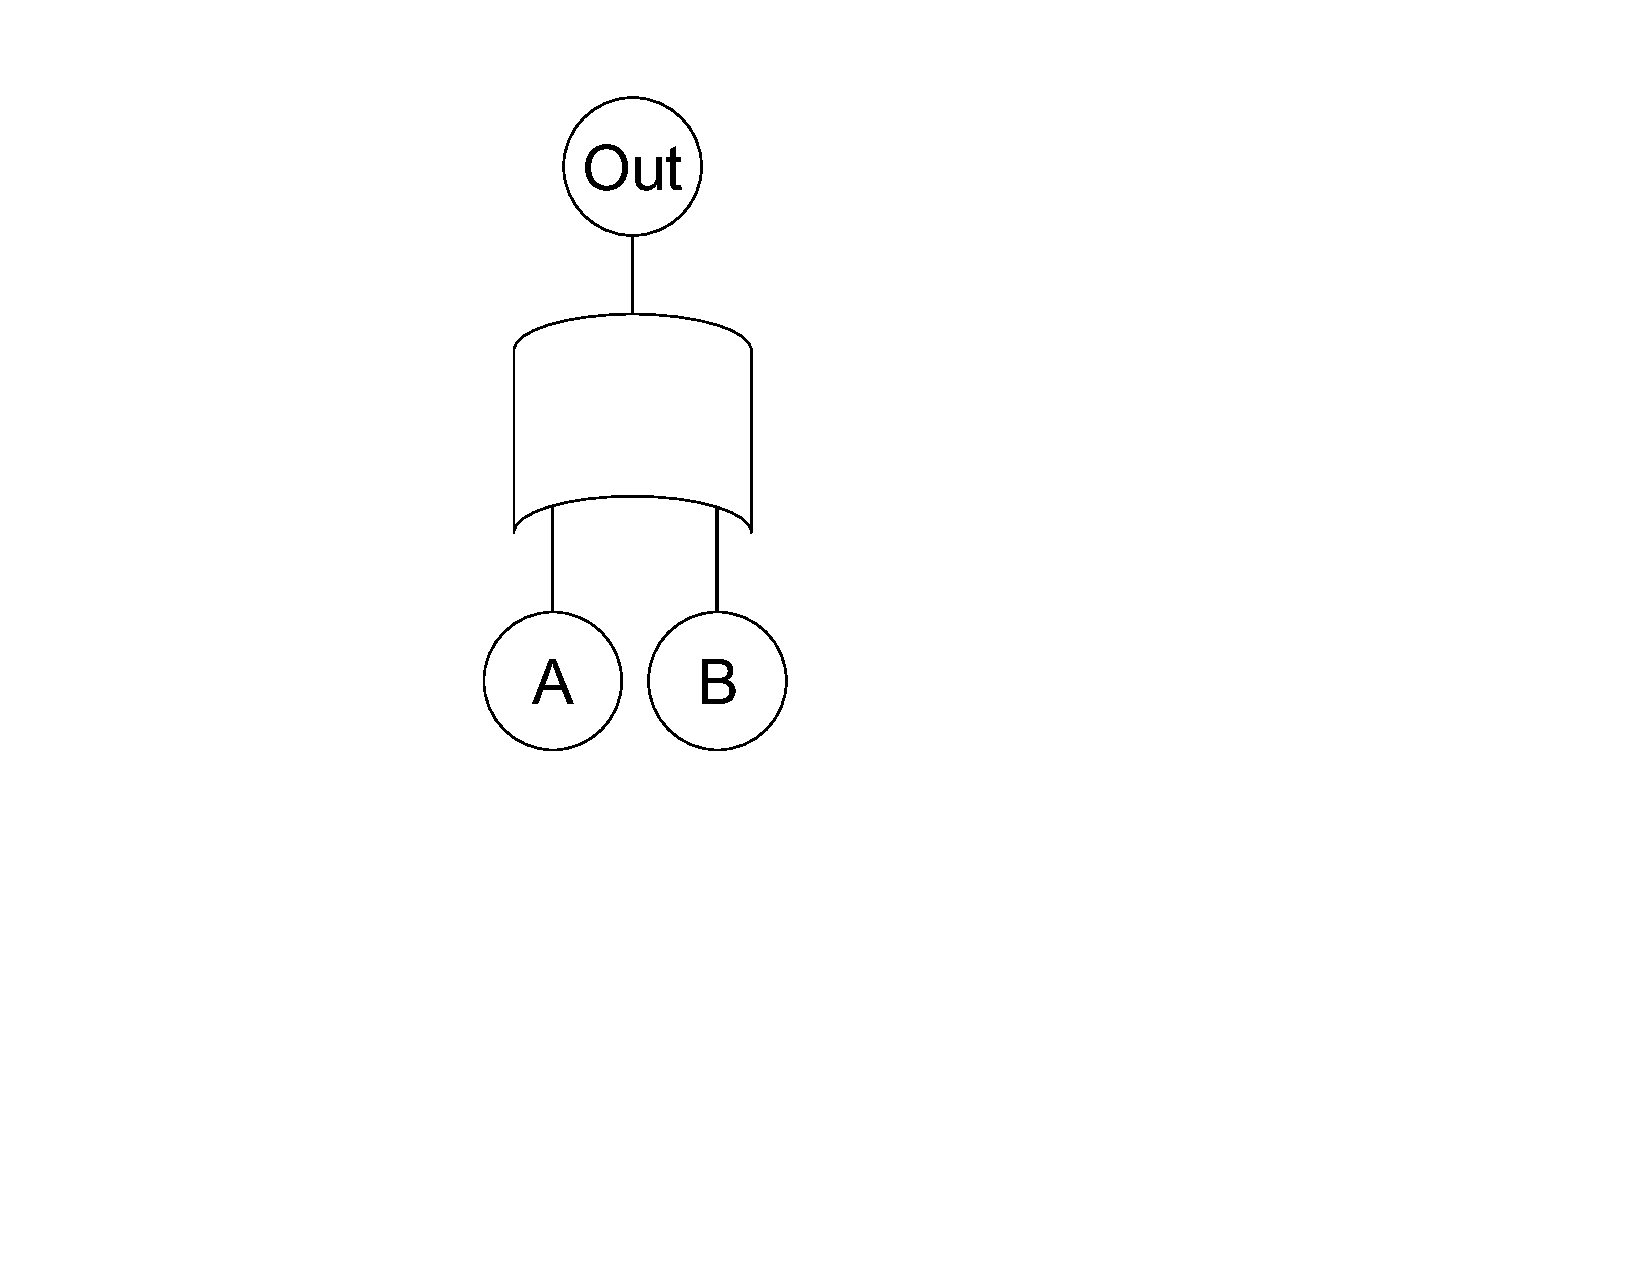
\includegraphics[scale=0.3]{andGate.pdf}
    \label{fig:andGate}
  \end{subfigure}
  \caption{Components A and B in a series configuration (left) and its associated Fault-Tree (right).}
  \label{fig:ABsystem}
\end{figure}

\begin{figure}
    \centering
    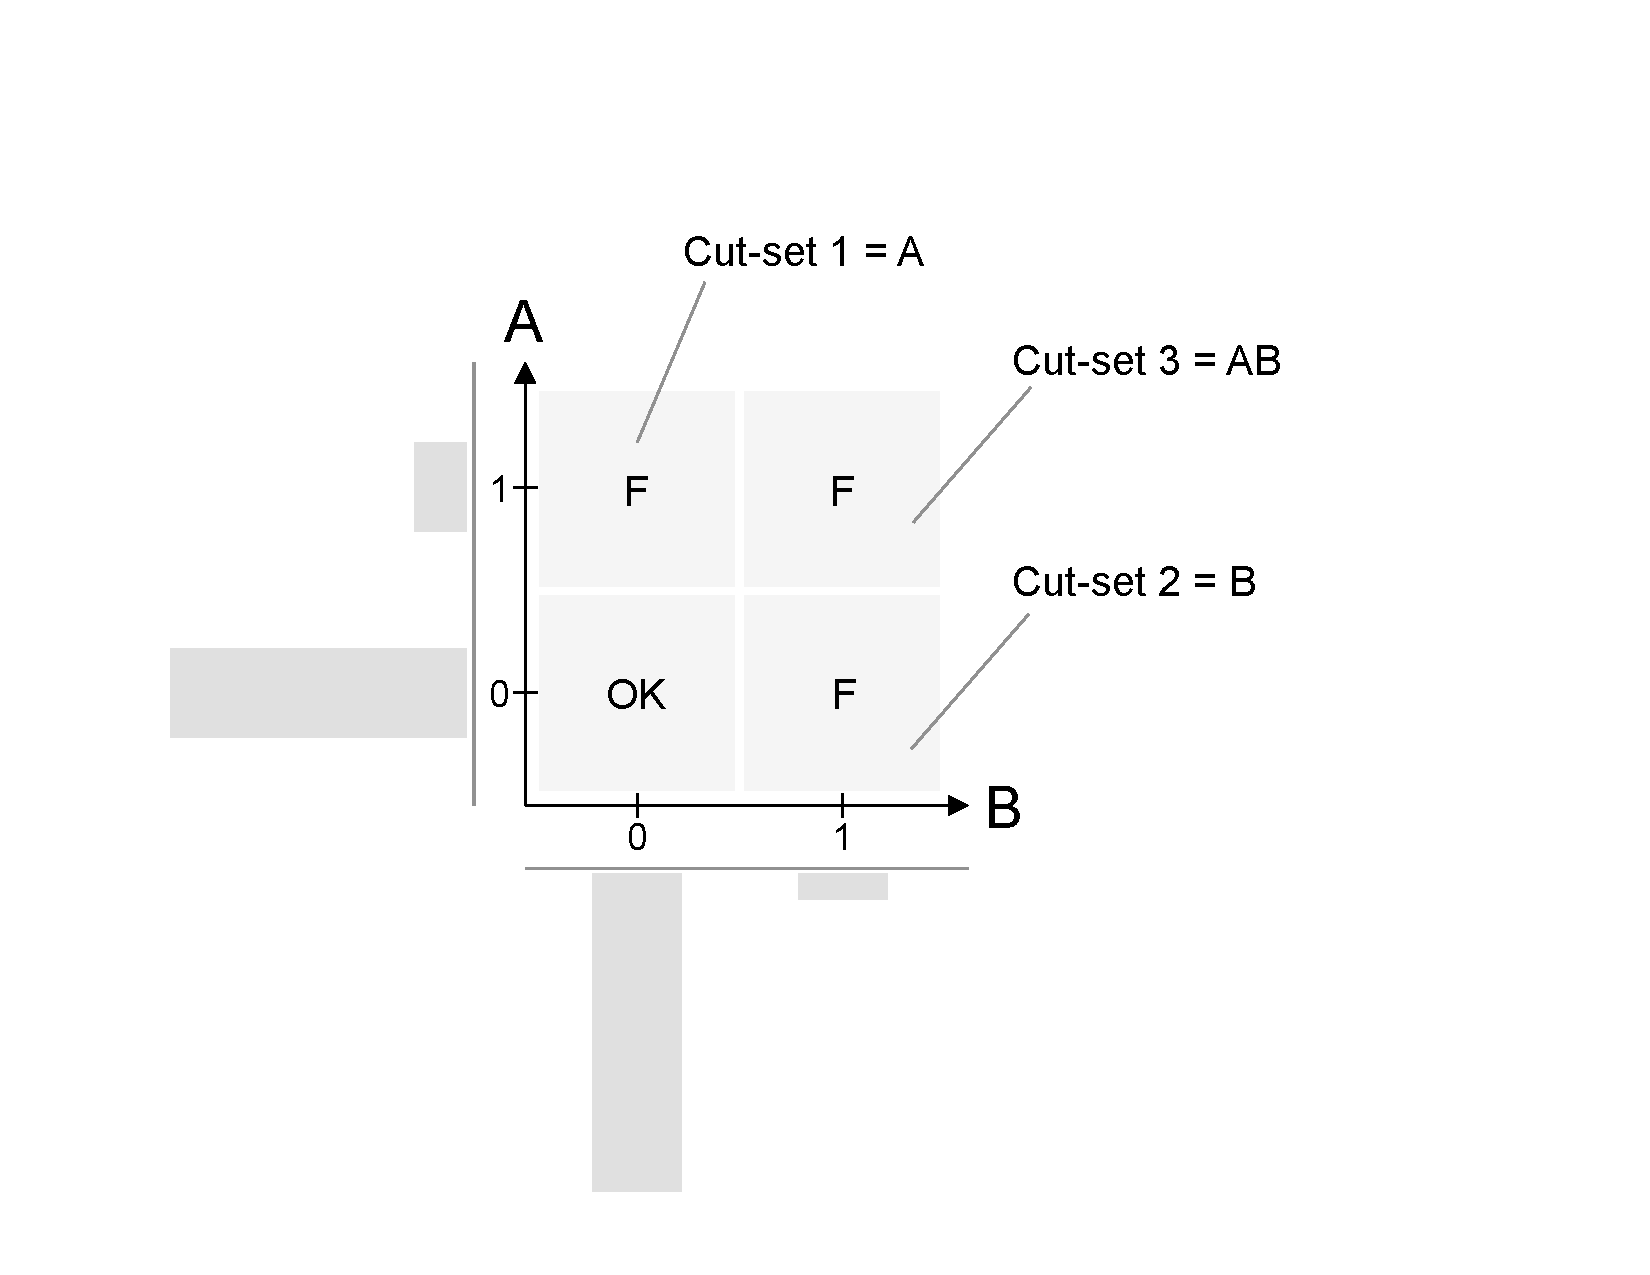
\includegraphics[scale=0.6]{2D.pdf}
    \caption{}
    \label{fig:2Danalogy}
\end{figure} 

\subsection{Example 1: series/parallel configuration}
\label{sec:example1}

The first example consists of 3 components 
arranged in a series/parallel configuration as shown in Fig.~\ref{fig:example12}. 
In this case the following probabilities of failures (on-demand) are provided:
\begin{itemize}
  \item $p_A = 1.0 \cdot 10^{-2}$
  \item $p_B = 5.0 \cdot 10^{-2}$
  \item $p_C = 1.0 \cdot 10^{-1}$
\end{itemize}

\begin{figure}
    \centering
    \centerline{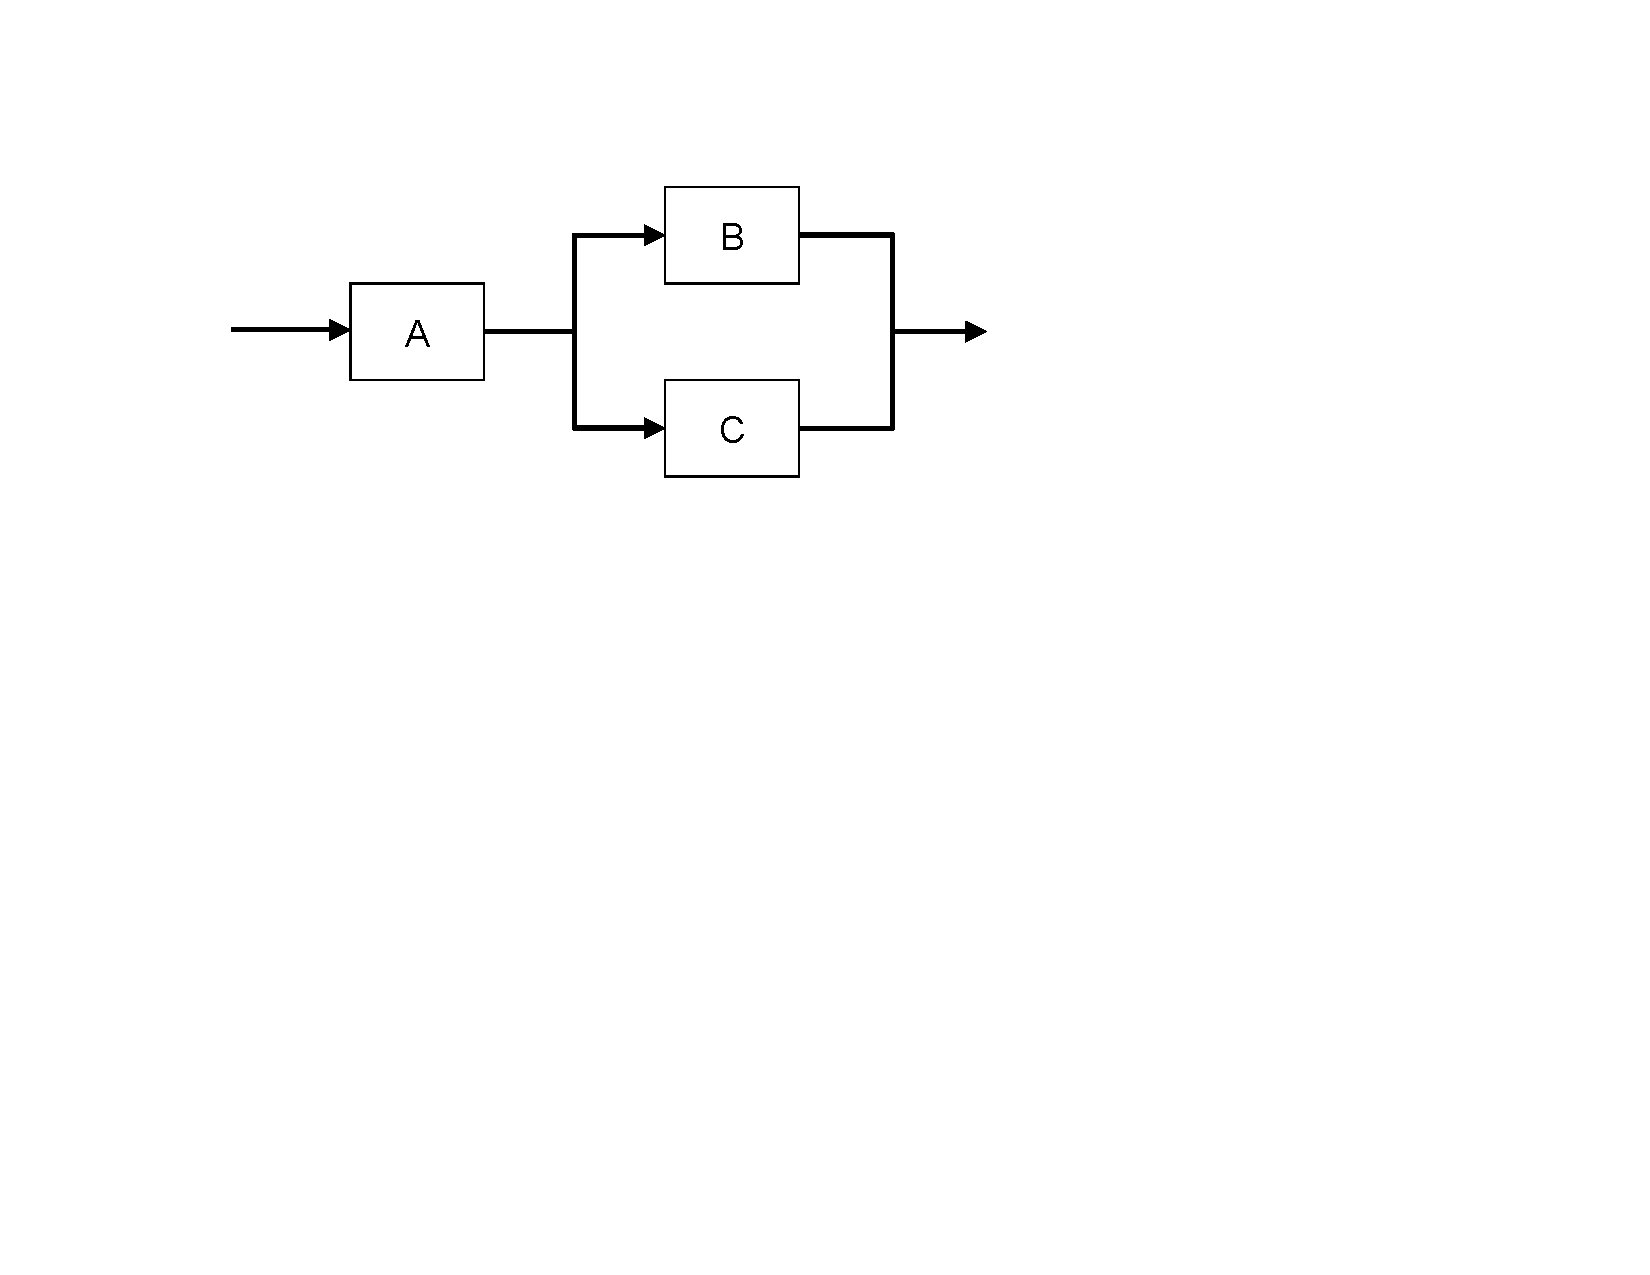
\includegraphics[scale=0.6]{simpleCase.pdf}}
    \caption{System considered for Examples 1 and 2.}
    \label{fig:example12}
\end{figure}

From a classical PRA perspective, this system can be modeled using a FT as shown in Fig.~\ref{fig:case1_FT}.

\begin{figure}
    \centering
    \centerline{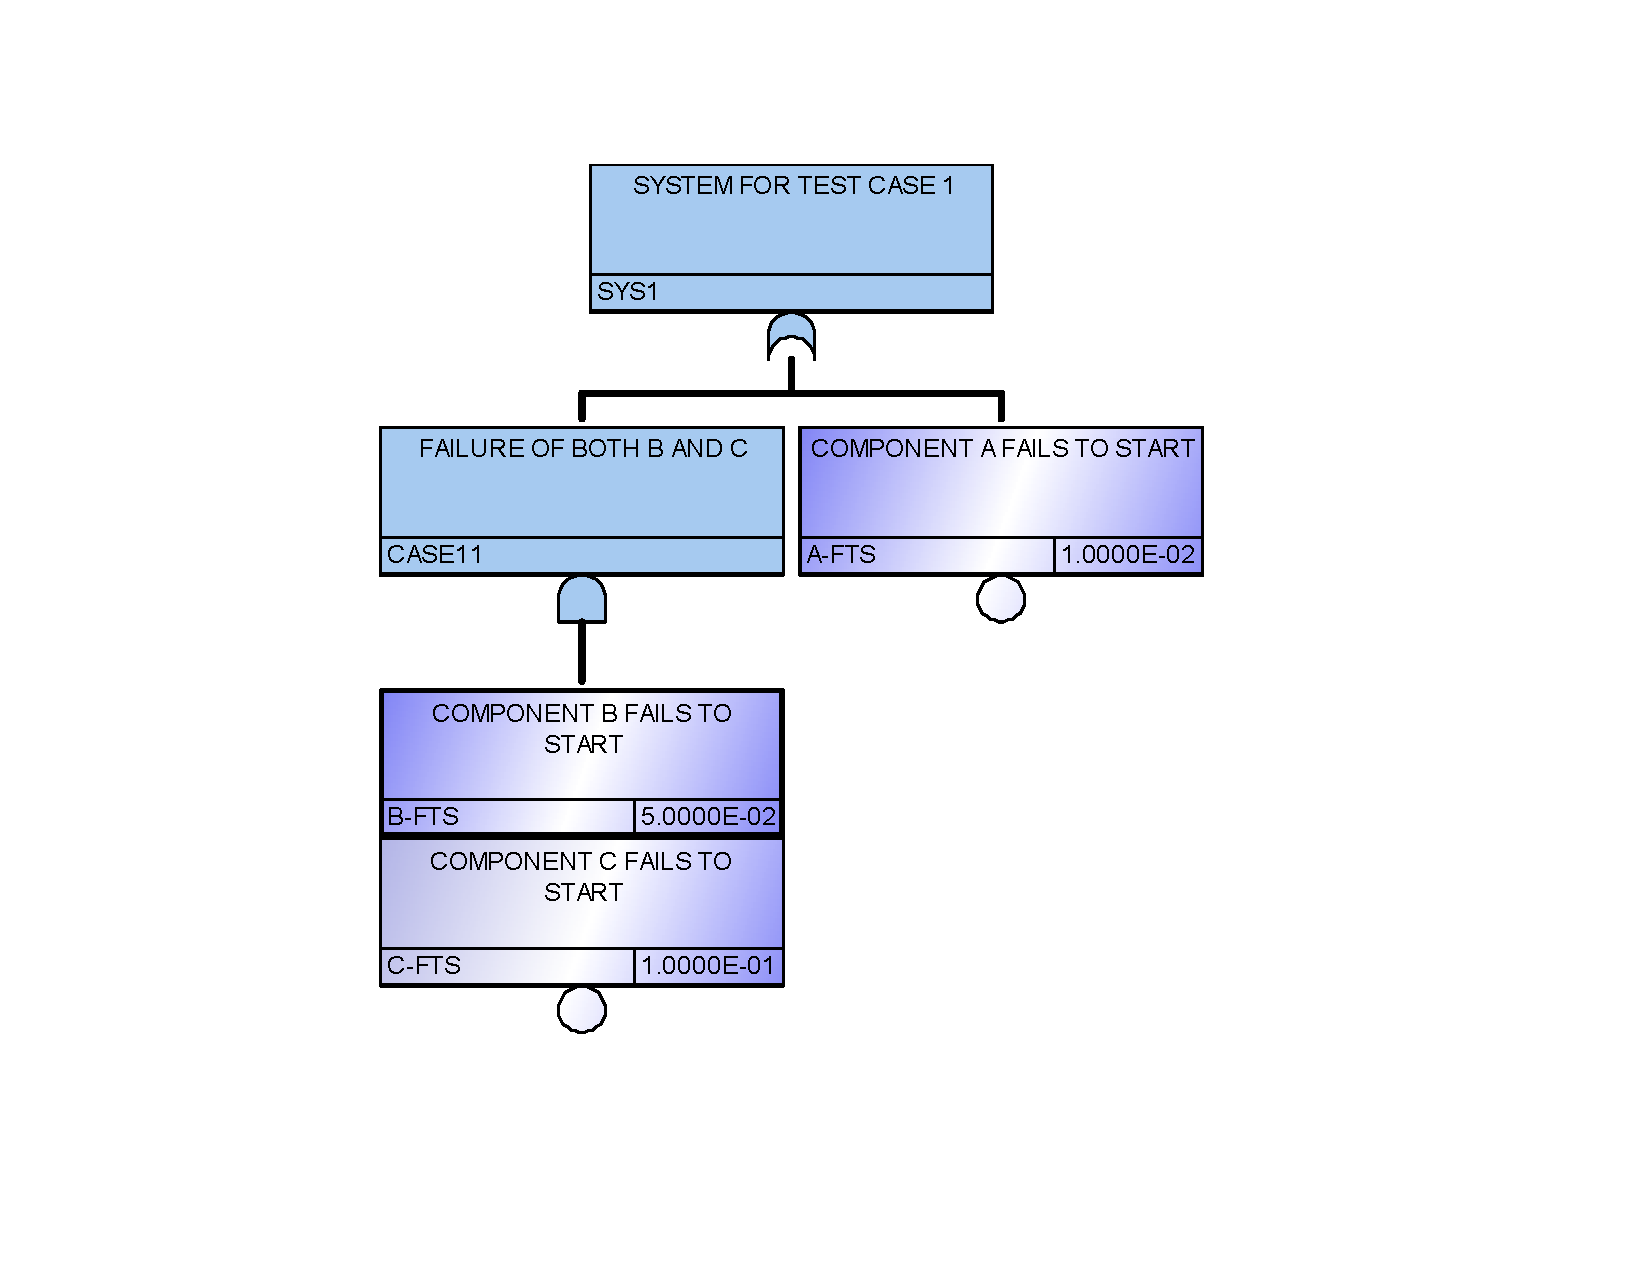
\includegraphics[scale=0.4]{case1_FT.pdf}}
    \caption{FT structure for the system shown in Fig.~\ref{fig:example12}.}
    \label{fig:case1_FT}
\end{figure}
  
From a RISMC (i.e., dynamic PRA) point of view the analysis of this system is performed as 
follows (see Section~\ref{sec:analogy}):
\begin{itemize}
  \item Define 3 stochastic parameters (i.e., $S=3$):
    \begin{itemize}
      \item $s_1$: status of component A
      \item $s_2$: status of component B
      \item $s_3$: status of component C
    \end{itemize}
  \item Assign a distribution to each stochastic parameter; in this case a Bernoulli 
        distribution  
  \item Define $I_i^+$ and $I_i^-$ for each distribution: in this case we have chosen 
        $I_i^-=[0.0,0.1]$ and $I_i^+=[1.0,1.1]$ 
  \item Generate $N$ samples, for example by employing Monte-Carlo or Grid sampling strategies
  \item Determine $R_0$, $R_i^-$ and $R_i^+$ for each component 
  \item Determine the desired RIMs for each component
\end{itemize}

Note that a Monte-Carlo sampling is not the best sampling strategy in terms of computational 
costs. This is even more relevant if the value of $p_A$, $p_B$ or $p_C$ were several order of 
magnitude lower. 

A more effective sampling strategy would be the Grid sampling (see Section~\ref{sec:analogy}): 
the stochastic variables 
are sampled over a fixed Cartesian grid and a probability weight is associated to each sample. 
In this case, each stochastic variable $s_i$ is sampled over two values, 0.0 and 1.0, and the 
probability weights $w_i^0$ and $w_i^1$ values associated to each sample coordinate are:
\begin{itemize}
  \item $s_i=0.0$: $w_i^0=prob(s_i \in [-\infty,0.5])$
  \item $s_i=1.0$: $w_i^1=prob(s_i \in [0.5,+\infty])$
\end{itemize}
Following this grid sampling strategy, only $2^3=8$ are needed.
Table~\ref{tab:example1}, the FV and RAW importance values for all three components obtained by RAVEN (using a 
Grid sampling strategy) are shown compared with the analytical ones.

\begin{table}
    \caption{Results obtained for Example 1.}
    \centering
    \begin{minipage}{.5\linewidth}
      \centering
      \begin{tabular}{c | c | c | c} 
        \hline 
         & Analytical & SAPHIRE & RAVEN \\ 
        \hline 
        $FV_A$ & 0.67 & 0.67 & 0.67  \\
        $FV_B$ & 0.33 & 0.34 & 0.33   \\
        $FV_C$ & 0.33 & 0.34 & 0.33   \\
        \hline 
      \end{tabular}
    \end{minipage} \\[2ex] 
    \begin{minipage}{.5\linewidth}
      \centering
      \begin{tabular}{c | c | c | c} 
        \hline 
         & Analytical & SAPHIRE & RAVEN \\ 
        \hline 
        $RAW_A$ & 66.9  & 66.9 & 66.9  \\
        $RAW_B$ & 7.3  & 7.3 & 7.3   \\
        $RAW_C$ & 3.98 & 3.98 & 3.98   \\
        \hline 
      \end{tabular}
    \end{minipage} 
    \label{tab:example1}
\end{table}

% 
% \subsection{Example 2: Time-dependent system}
% \label{sec:example2}
% 
% The second example is similar to Example I but with different reliability data: 
% a failure rate is provided for each component (mission time: 24 hours): 
% \begin{itemize}
%   \item $\lambda_A = 1.0 10^{-3} hr^{-1}$
%   \item $\lambda_B = 5.0 10^{-3} hr^{-1}$
%   \item $\lambda_C = 1.0 10^{-2} hr^{-1}$
% \end{itemize}
% Thus it is assumed that failure probability of each component is exponentially 
% distributed: sampled value $s_i$ from its own distribution is failure time of each 
% component ($t_A$, $t_B$ and $t_C$).
% In this case, $I_i^+$ and $I_i^-$ can be defined as follows:
% \begin{itemize}
%   \item $I_i^-=[24.0,+\infty]$: component is considered perfectly reliable if the failure 
%         time is greater than the mission time
%   \item $I_i^+=[0.0,1.0]$: component is considered unreliable if the failure time 
%         occurs within the first hour
% \end{itemize}
% 
% As shown for Example I, a Grid sampling strategy has been employed. Table~\ref{} shows the 
% FV importance for all three components obtained by RAVEN (using a Grid sampling strategy) 
% compared with the analytical ones.
% 
% \begin{table}
%   \caption{Results obtained for Example II.} 
%   \centering 
%   \begin{tabular}{c | c | c } 
%     \hline 
%      & Analytical & RAVEN \\ 
%     \hline 
%     $FV_A$ & 0.48957 & 0.48957  \\
%     $FV_B$ & 0.4983  & 0.4983   \\
%     $FV_C$ & 0.4983  & 0.4983   \\
%     \hline 
%   \end{tabular}
%   \label{tab:example2} 
% \end{table}

\subsection{Example 2: time-dependent stand-by configuration}
\label{sec:example2}

The second example considers a simplified ECCS model (see Fig.~\ref{}) of a reactor. 
It consists of the following components and for a subset of them a 
value of mean time to failure (MTTF) is provided:
\begin{itemize}
  \item Motor-operate valve M (MTTF = 24 h, $\lambda_{valve} = 0.041667$)
  \item Two redundant pumps, pump1 and pump2 
        (MTTF = 12 h, $\lambda_{pump1} = \lambda_{pump2} = 0.083333$)
  \item Heat exchanger HX (reliability = 1.0)
\end{itemize}

Pump1 is normally used while pump2 is on standby. If Pump1 fails then pump2 provide water flow 
in a switching arrangement. 
Pump2 cannot fail while in standby. Switch from pump1 to pump2 is perfectly reliable. 
The cooling is such that it takes 2 hours to reach vessel failure condition if the 
M-pump1-pump2 
system has failed. Mission time is again equal to 24 hours.

\begin{figure}
    \centering
    \centerline{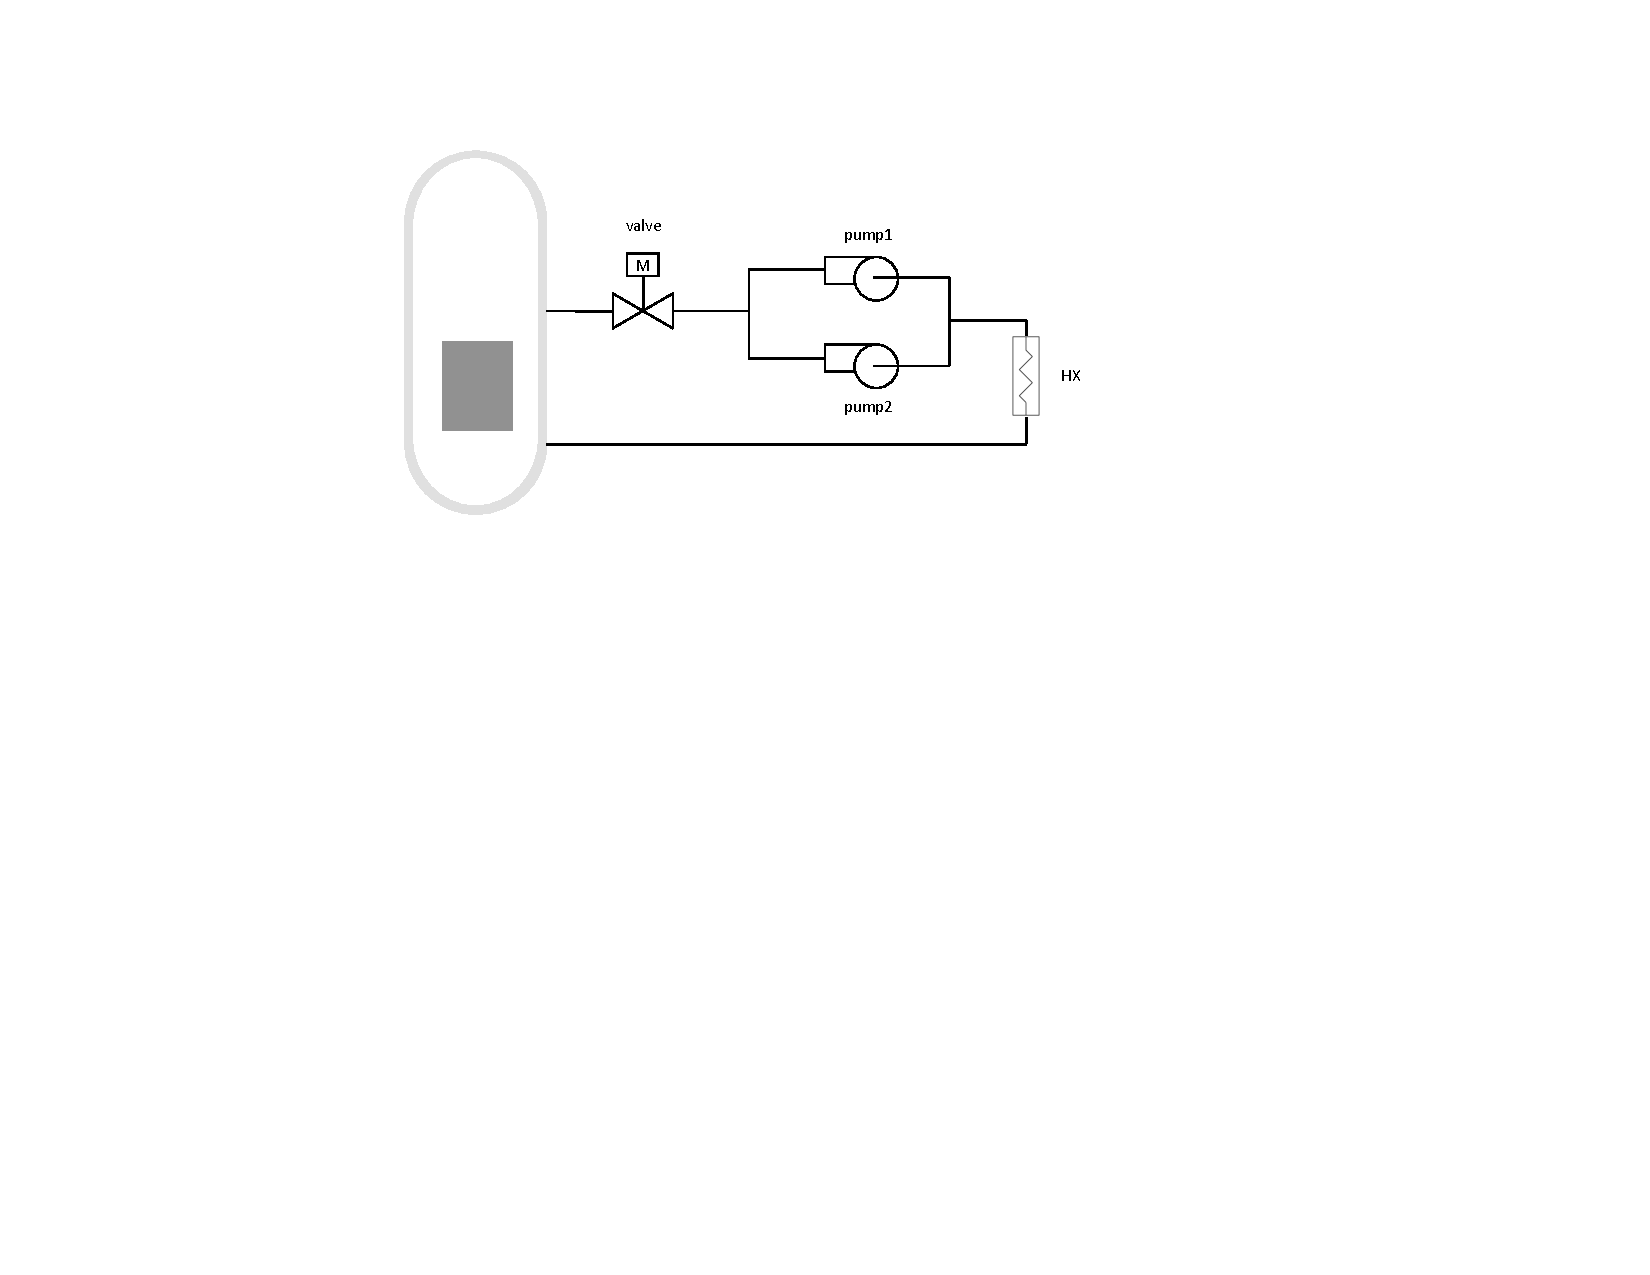
\includegraphics[scale=0.6]{case2.pdf}}
    \caption{System considered for Example 3.}
    \label{fig:example3}
\end{figure}

Note in this case classical PRA methods require model adjustments via convolution calculations
in order to correctly 
determine system reliability.
Table~\ref{tab:example2} are shown the FV importance for all three components obtained by RAVEN (using a Monte-Carlo 
sampling strategy) compared with the analytical ones.

\begin{table}
    \centering
    \caption{Results obtained for Example 2.}
    \begin{minipage}{.5\linewidth}
      \centering
      \begin{tabular}{c | c | c | c} 
        \hline 
         & Analytical & SAPHIRE & RAVEN \\ 
        \hline 
        $FV_{valve}$ & 0.30 & 0.69 & 0.30 \\
        $FV_{pump1}$ & 0.26 & 0.82 & 0.26 \\
        $FV_{pump2}$ & 0.26 & 0.82 & 0.26 \\
        \hline 
      \end{tabular}
    \end{minipage} \\[2ex]
    \begin{minipage}{.5\linewidth}
      \centering
      \begin{tabular}{c | c | c | c} 
        \hline 
         & Analytical & SAPHIRE & RAVEN \\ 
        \hline 
        $RAW_{valve}$ & 1.18 & 1.10 & 1.18 \\
        $RAW_{pump1}$ & 1.12 & 1.05 & 1.12 \\
        $RAW_{pump2}$ & 1.12 & 1.05 & 1.12 \\
        \hline 
      \end{tabular}
    \end{minipage} 
    \label{tab:example2}
\end{table}


\subsection{Example 3: $K$ out of $N$ configuration}
\label{sec:example3}

The third example is similar to the one shown in Section~\ref{sec:example2}
It consists of the following components:
\begin{itemize}
  \item Motor-operate valve M (MTTF = 24 h, $\lambda_{valve} = 0.041667$)
  \item Three pumps, pump1, pump2 and pump3 
        (MTTF = 12 h, $\lambda_{pump1} = \lambda_{pump2} = \lambda_{pump3} = 0.083333$)
  \item Heat exchanger HX (reliability = 1.0)
\end{itemize}
All pumps are initially running but 2 out of 3 are required to cool the system.
Mission time is again equal to 24 hours.

\begin{figure}
    \centering
    \centerline{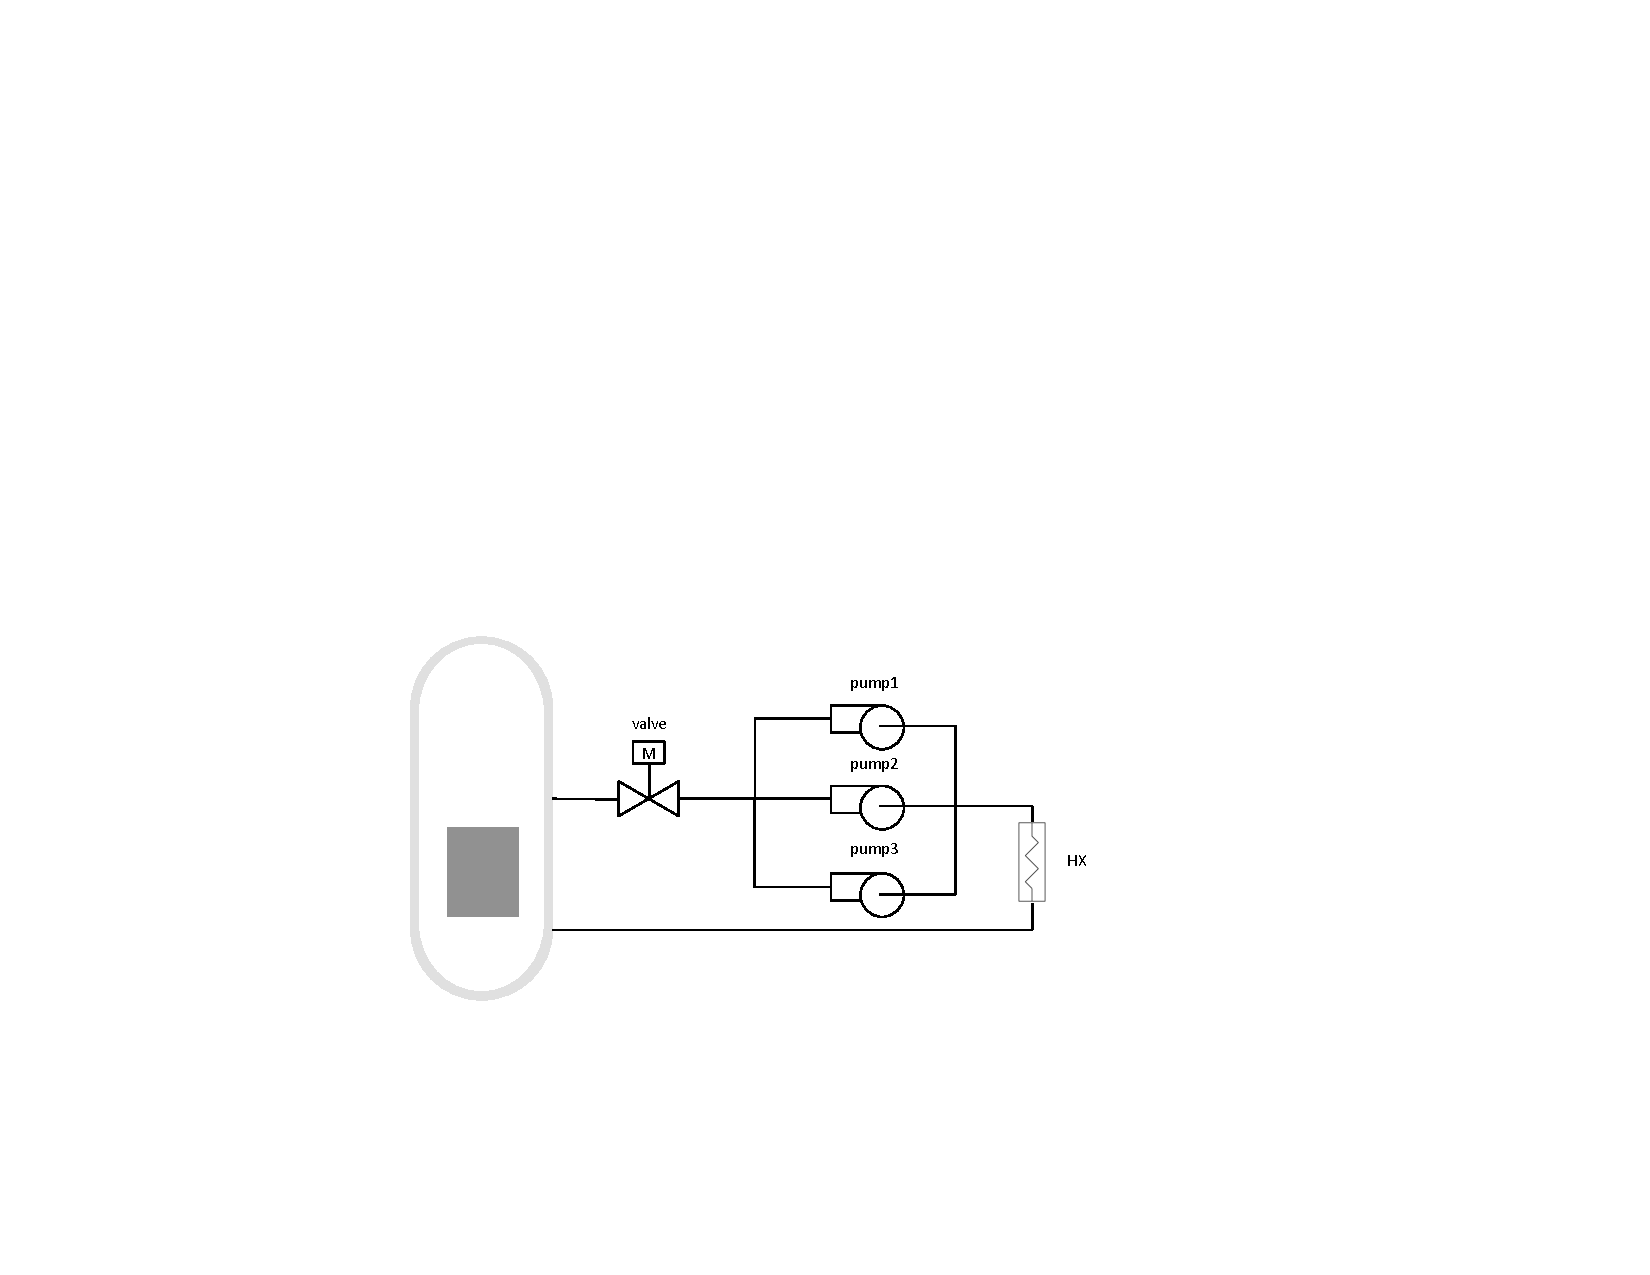
\includegraphics[scale=0.6]{case3.pdf}}
    \caption{System considered for Example 3.}
    \label{fig:example4}
\end{figure}

Table~\ref{tab:example3} are shown the FV importance for all three components obtained by RAVEN (using a Monte-Carlo 
sampling strategy) compared with the analytical ones.

\begin{table}
    \centering
    \caption{Results obtained for Example III.}
    \begin{minipage}{.5\linewidth}
      \centering
      \begin{tabular}{c | c | c | c} 
        \hline 
         & Analytical & SAPHIRE & RAVEN \\ 
        \hline 
        $FV_{valve}$ & 0.032 & 0.64 & 0.033  \\
        $FV_{pump1}$ & 0.076 & 0.94 & 0.081  \\
        $FV_{pump2}$ & 0.076 & 0.94 & 0.081  \\
        $FV_{pump3}$ & 0.076 & 0.94 & 0.081  \\ 
        \hline 
      \end{tabular}
    \end{minipage} \\[2ex]
    \begin{minipage}{.5\linewidth}
      \centering
      \begin{tabular}{c | c | c | c} 
        \hline 
         & Analytical & SAPHIRE & RAVEN \\ 
        \hline 
        $RAW_{valve}$ & 1.02 & 1.0 & 1.02  \\
        $RAW_{pump1}$ & 1.01 & 1.0 & 1.01  \\
        $RAW_{pump2}$ & 1.01 & 1.0 & 1.01  \\
        $RAW_{pump3}$ & 1.01 & 1.0 & 1.01  \\ 
        \hline 
      \end{tabular}
    \end{minipage} 
    \label{tab:example3}
\end{table}


\subsection{Example 4: time and physics dependent stand-by configuration}
\label{sec:example4}

The forth example considers the system of Example 2 (see Section~\ref{sec:example2}) but it considers 
also the temporal behavior of the reactor.
The top event is not the failure of valve-pump1-pump2 system but it occurs when core temperature $T$
reaches a threshold value $T_{max}$ (i.e., reactor failure). 
Mission time is still 24 hours.

Note that the configuration is slightly different from the one presented in the first two 
examples (here a stand-by configuration is introduced) but also the condition of system failure 
is dictated by the dynamic behavior of the PWR. The system is designed such that a late failure 
of the ECCS may not lead to system failure (i.e., natural circulation is providing enough cooling). 
In other words, the ECCS is vital especially in the hours right after a reactor scram.

In principle, this test case cannot be solved analytically due to the complexity of the reactor 
behavior. It can be solved by identifying the time $T_{lim}$ (limit time) after which a 
failure of the valve-pump1-pump2 system does not cause reactor failure since natural circulation
can provide enough cooling.
Note that $T_{lim}$ could only be determined be recursively run the system simulator until a 
good estimate of $T_{lim}$ is reached.

Figure~\ref{fig:limitTime} shows the histogram of the failure time of valve-pump1-pump2 system along 
with the limit time $T_{lim}$ for the two different power levels (100\% and 120\%). 
Note that a higher power level implies a faster reactor heatup rate; hence, the 
valve-pump1-pump2 system must provide more cooling before the natural circulation can sustain a failure
of the valve-pump1-pump2 system: $T_{lim}$ increases.

\begin{figure}
    \centering
    \centerline{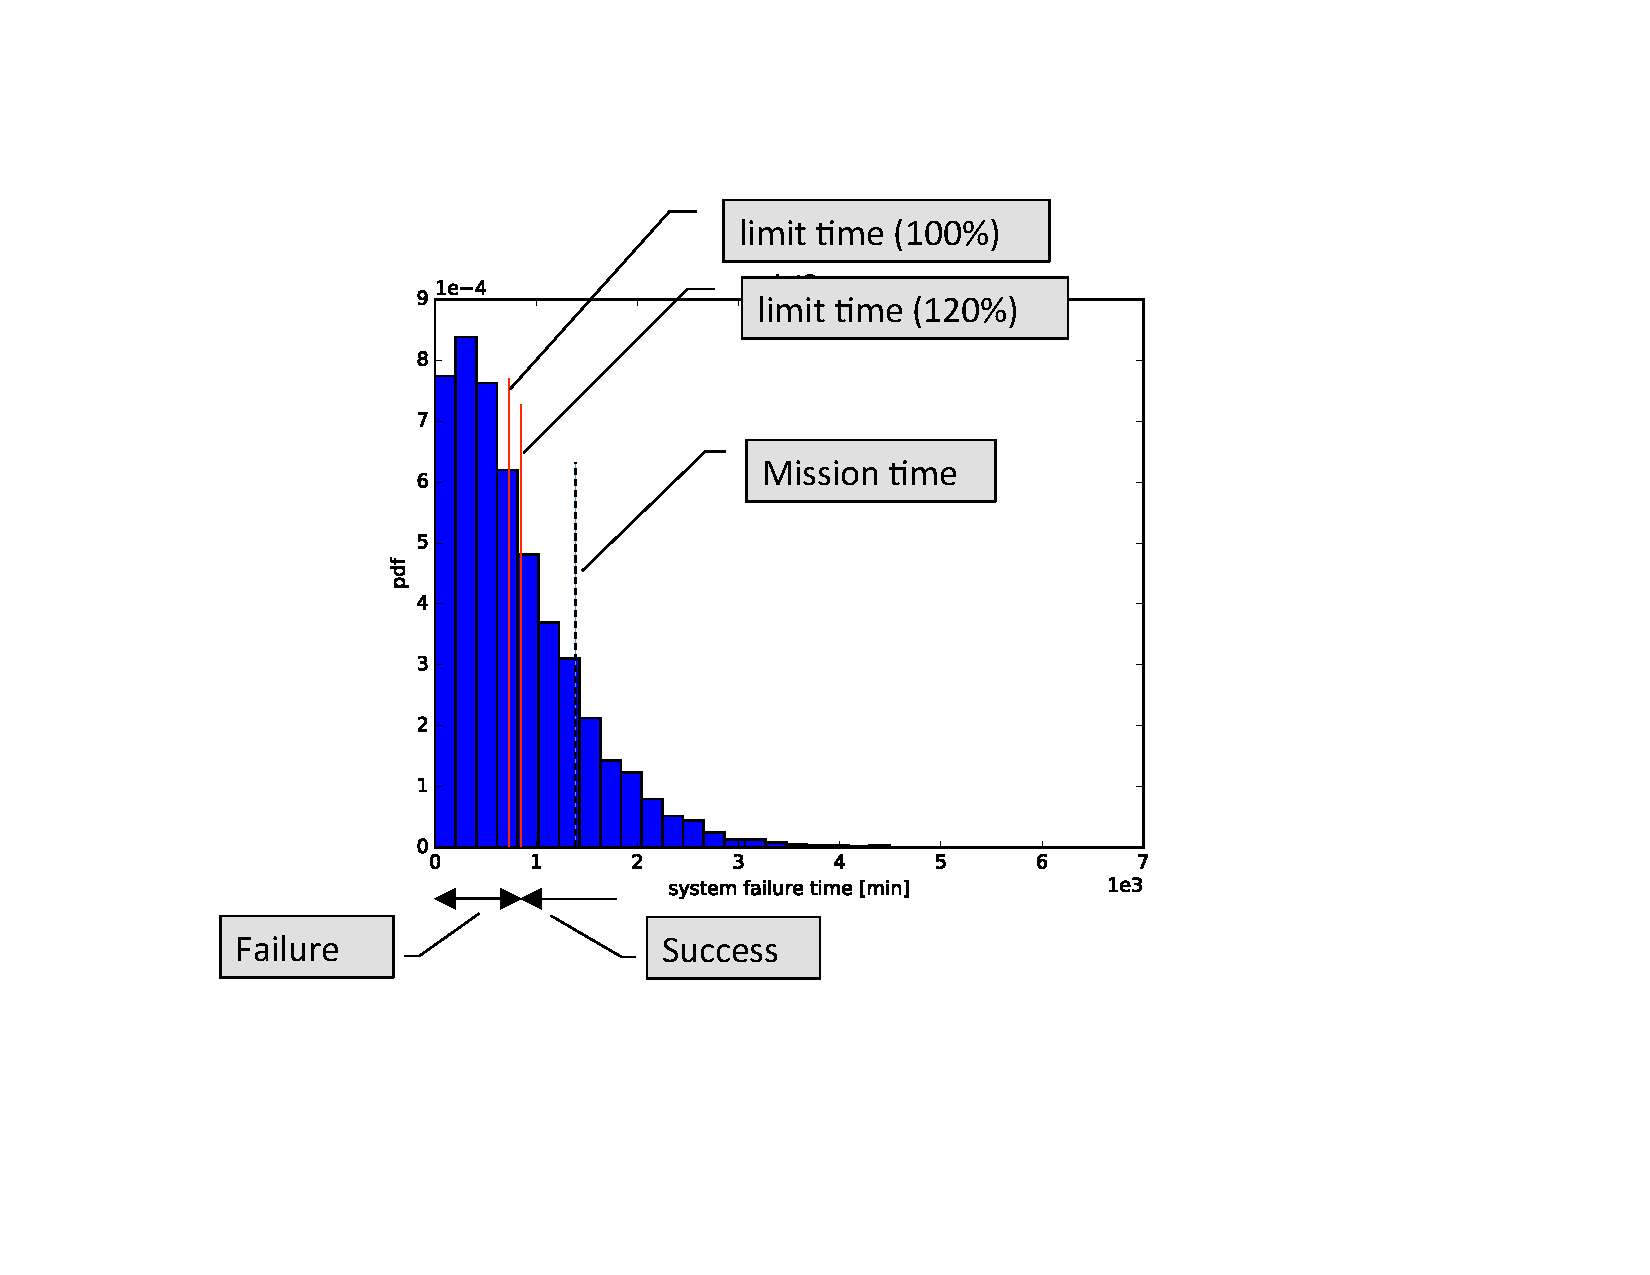
\includegraphics[scale=0.4]{limitTime.pdf}}
    \caption{}
    \label{fig:limitTime}
\end{figure}

\begin{table}
  \caption{Results obtained for Example 4.}
  \centering
  \begin{tabular}{c | c | c }
    \hline
          & FV & RAW \\
    \hline
    valve & 0.58 & 2.21  \\
    pump1 & 0.28 & 1.48  \\
    pump2 & 0.28 & 1.48  \\
    \hline
  \end{tabular}
  \label{tab:example4}
\end{table}

\subsubsection{Considerations on the mission time}
\label{sec:missionTime}

In the example presented in Section~\ref{sec:example4} two code stopping conditions were: core temperature 
greater than 2200 F and simulation time reaches 24 hours (mission time).
Note that the mission time stopping condition imposes that a simulation is considered successful even if the
valve-pump1-pump2 system has failed and the reactor temperature increases; if a longer mission time would 
be chosen then the simulation would be classified no longer with an OK outcome but with a fail outcome.
Thus, special attention has be given to the assumptions behind the mission time. 

Depending on the employed code simulator the best solution is to re-define the mission time $T_{miss}$ as the 
time below which events can occur; in addition, the code is set to end the simulation not when the mission 
time is reached but at a time $T_{end} = T_{miss} + T_{relax}$ where the addition of $T_{relax}$ allows 
the simulation to reach a steady-state condition.

\subsubsection{Considerations on the sampling strategy}
\label{sec:samplingStrategy}

In order to get accurate results of the risk importance measures the number of simulation runs to perform 
can be very high (order of thousands and up). In addition, given that each simulation run may require 
hours of simulation time, this kind of analysis may be feasible only for large high performance computing 
systems.

An alternative approach is to employ ROMs instead of the actual simulation code so that a large number of 
data points can be generated in a much faster time on standard computing machines.
In this case the approach would be as follows:
\begin{enumerate}
  \item Generate a limited set of sample points using the simulation code 
  \item Train and validate a ROM given the data set generated in Step 1
  \item Perform the analysis with the ROM obtained in Step 2
\end{enumerate}
The training and creation of the ROM can be performed in several ways; for the applications targeted by this 
paper we have found two optimal choices.

The first one explores the totality of input space uniformly and it reconstructs the response of the code in 
the input space. 

The second one exploits the binary nature of the problem (i.e., the outcome of each simulation run is binary:
either OK or failed) and it try to determine the limit surface: the boundaries in the input space that separate 
failure region (i.e.,
characterized by the undesired simulation outcome; e.g., core damage) from success region (i.e., characterized 
by the desired simulation outcome; e.g., max clad temperature below 2200 F). 
This sampling strategy, called ``adaptive sampling'' (or smart sampling), can obtain much better statistical results
since the the code response is queried in the most relevant zones of the input space (the limit surface).

The steps for the adaptive sampling strategy are:
\begin{enumerate}
  \item Perform a set of runs of the simulator code: the number of required runs may depend on the dimensionality of 
        the input space
  \item Given the set of simulation runs obtained in Step 1, create a ROM. The objective of this ROM is to infer the 
        response of the simulator code, i.e., create an approximate output given the same set of input parameters
  \item Identify a set of points on the limit surface
  \item Chose a subset of points from the ones obtained in Step 4 
  \item Perform a simulation run for each of the points obtained in Step 5 using the simulator code
  \item Repeat Steps 2 through 6 until convergence is reached
\end{enumerate}

An example of adaptive sampling is shown in Fig.~\ref{fig:adaptiveSampling} for a 2-dimensional case. 
Figure~\ref{fig:adaptiveSampling} shows
the location of the chosen sample points and the estimate of the limit surface as the iteration illustrated above 
progresses. Note that the code is evaluated in a safety strategic area: the limit surface. 

\begin{figure}
    \centering
    \centerline{\includegraphics[scale=0.55]{adaptiveSampling.pdf}}
    \caption{Example of adaptive sampling}
    \label{fig:adaptiveSampling}
\end{figure}

   

 


